\documentclass[10pt,aspectratio=169]{beamer}
\usepackage[utf8]{inputenc}
\usepackage[french]{babel}
\usepackage[T1]{fontenc}
\usepackage{graphicx}
\usepackage{tikz}
\usepackage{xcolor}
\usepackage{fontawesome5}
\usepackage{listings}
\usepackage{tabularx}    % Pour la largeur automatique
\usepackage{booktabs}    % Pour les lignes de séparation (\toprule, etc.)
\usetikzlibrary{shapes.geometric,shapes.symbols,positioning,arrows.meta}
\usepackage{pgfplots}
\pgfplotsset{compat=1.18}
\usepackage{hyperref}
\usepackage{amsmath}
\usepackage{amssymb}
\usepackage{multicol}

% Pour les couleurs dans le tableau (\rowcolor)
\usetikzlibrary{shadows, arrows.meta}
\usetikzlibrary{shapes.geometric}
\definecolor{fogblue}{RGB}{188, 202, 222}
\definecolor{fogyellow}{RGB}{245, 230, 180}
\definecolor{fogred}{RGB}{245, 190, 190}
\definecolor{foggreen}{RGB}{190, 225, 190}

% Configuration du thème
\usetheme{Madrid}
\usecolortheme{seahorse}
\setbeamertemplate{navigation symbols}{}
\setbeamertemplate{footline}[frame number]

% Couleurs personnalisées
\definecolor{androidgreen}{RGB}{61,220,132}
\definecolor{darkgreen}{RGB}{0,100,0}
\definecolor{lightgray}{RGB}{240,240,240}

% Configuration des listings pour le code
\lstset{
    language=Java,
    basicstyle=\ttfamily\tiny,
    keywordstyle=\color{blue}\bfseries,
    commentstyle=\color{green!50!black},
    stringstyle=\color{red},
    showspaces=false,
    showstringspaces=false,
    frame=single,
    rulecolor=\color{black},
    tabsize=2,
    breaklines=true,
    breakatwhitespace=false,
}
% Page de titre
\title{\textbf{Fog-Assisted Vehicular Fog Computing}}
\subtitle{Module : Fog \& Edge Computing}

\author{
\begin{tabular}{p{6.5cm} p{4.5cm}}
\textbf{Présenté par :} & \textbf{Encadré par :} \\[0.2cm]
Oussama BENYSSEF & Pr. K. Ahed \\
Abdessamad EL FATHI & \\
Mouad ASSARGUAL & \\
Youssef LAGRAMEZ &
\end{tabular}
}

\institute{
Master : Intelligence Artificielle Embarquée\\
Année Universitaire : 2025--2026
}

\date{}

\AtBeginSection[]
{
  \begin{frame}{Plan}
    \tableofcontents[currentsection]
  \end{frame}
}

\begin{document}

% Slide de titre avec logo
\begin{frame}[plain]
    \begin{center}
        \includegraphics[width=5cm]{logo.png}
    \end{center}
    \vspace{0.5cm}
    \titlepage
\end{frame}

% ============================================
% PLAN
% ============================================
\begin{frame}{Plan de la Pr\'esentation}
\tableofcontents
\end{frame}

% ############################################
% SECTION 1 : PROBLEMATIQUE
% ############################################
\section{Probl\'ematique}

\begin{frame}{Contexte : R\'eseaux V\'ehiculaires (VANET)}
\begin{columns}
\column{0.5\textwidth}
\textbf{D\'efinition :}
\begin{itemize}
    \item R\'eseau ad-hoc form\'e par v\'ehicules communicants
    \item Communications V2V, V2I, V2N, V2P
    \item Mobilit\'e \'elev\'ee (50-150 km/h)
    \item Topologie dynamique et \'eph\'em\`ere
\end{itemize}

\column{0.5\textwidth}
\textbf{Applications critiques :}
\begin{itemize}
    \item \'Evitement de collision ($<$ 10 ms)
    \item Gestion intelligente du trafic
    \item Conduite autonome coop\'erative
    \item Services d'urgence et s\'ecurit\'e
\end{itemize}
\end{columns}

\vspace{0.3cm}
\begin{alertblock}{Exigences temps r\'eel}
S\'ecurit\'e routi\`ere : $<$ 20 ms \quad|\quad Gestion trafic : $<$ 100 ms \quad|\quad Fiabilit\'e : 99.999\%
\end{alertblock}
\end{frame}

\begin{frame}{D\'efis et Limites du Cloud Computing}
\begin{columns}
\column{0.5\textwidth}
\textbf{D\'efis des VANET :}
\begin{itemize}
    \item \textcolor{fogred}{Congestion r\'eseau} : Pics de trafic en heures de pointe
    \item \textcolor{fogred}{Latence \'elev\'ee} : 100-250 ms via Cloud
    \item \textcolor{fogred}{Surcharge Cloud} : Centralisation des calculs
    \item Bande passante limit\'ee (V2I)
    \item Mobilit\'e rapide des n\oe uds
\end{itemize}

\column{0.5\textwidth}
\textbf{Limites du Cloud seul :}
\begin{itemize}
    \item[$\times$] RTT trop \'elev\'e ($\sim$250 ms)
    \item[$\times$] Point unique de d\'efaillance
    \item[$\times$] Co\^uts de bande passante \'elev\'es
    \item[$\times$] Pas de conscience du contexte local
    \item[$\times$] Inadapt\'e au temps r\'eel v\'ehiculaire
\end{itemize}
\end{columns}

\vspace{0.3cm}
\begin{block}{Constat}
Le Cloud seul \textbf{ne peut pas} r\'epondre aux exigences de latence des applications v\'ehiculaires temps r\'eel. Il faut rapprocher le calcul des v\'ehicules.
\end{block}
\end{frame}

% ############################################
% SECTION 2 : OBJECTIF PRINCIPAL
% ############################################
\section{Objectif Principal}

\begin{frame}{Objectif du Projet}
\textbf{Objectif principal :}
\begin{enumerate}
    \item \textbf{G\'erer la congestion} du trafic routier en temps r\'eel via Fog Computing
    \item \textbf{Optimiser le task offloading} dans un environnement v\'ehiculaire multi-tiers
    \item \textbf{D\'emontrer l'apport} du Fog/Edge Computing par rapport au Cloud seul
\end{enumerate}

\vspace{0.1cm}
\textbf{Architecture 3-tiers propos\'ee :}
\begin{center}
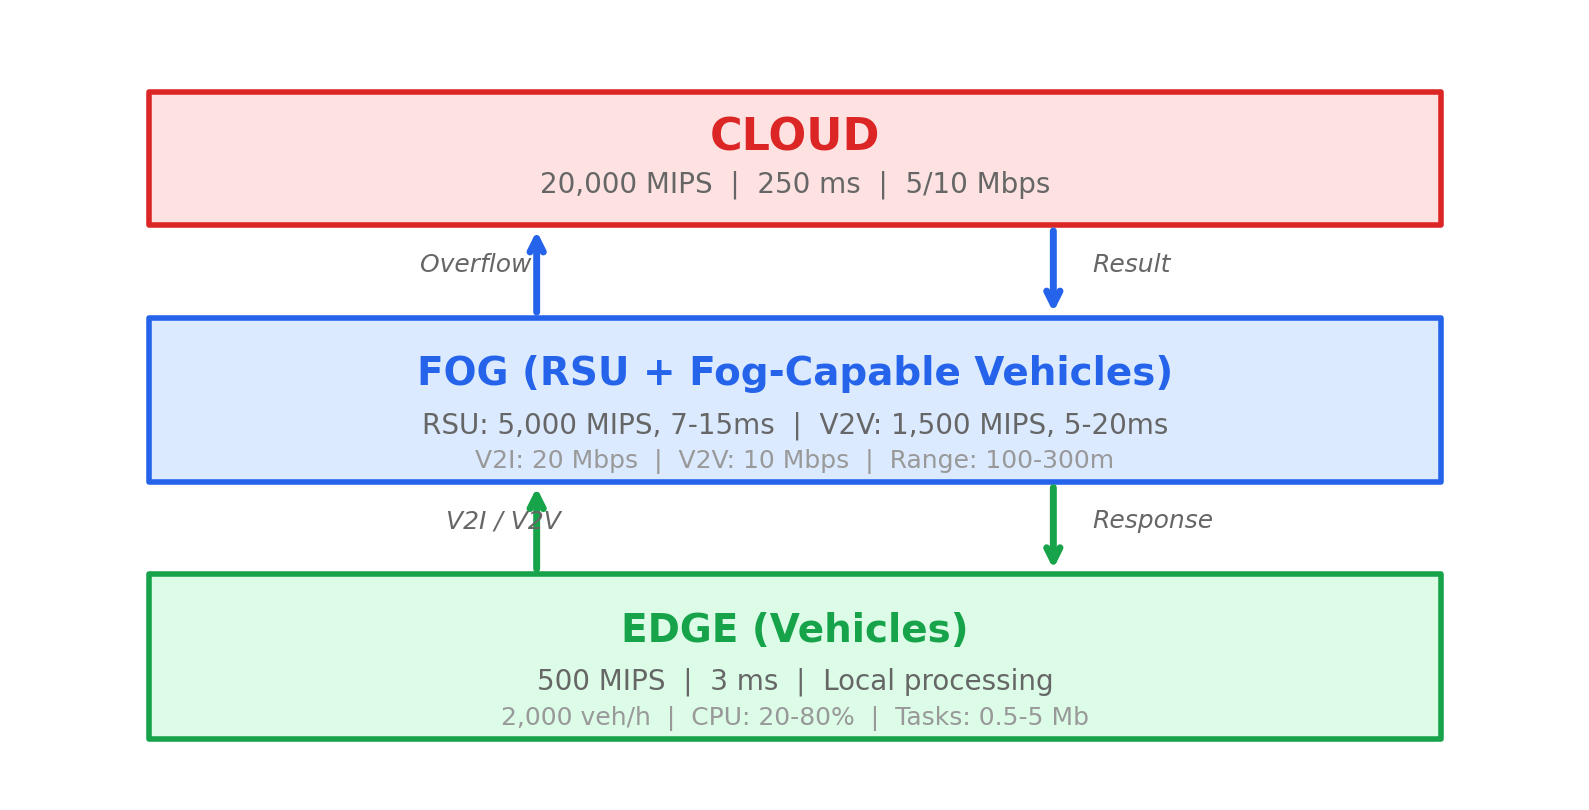
\includegraphics[width=0.9\textwidth,height=0.40\textheight,keepaspectratio]{plot5_architecture.png}
\end{center}

\begin{block}{R\'esultat cl\'e}
R\'eduction de latence jusqu'\`a \textbf{80\%} gr\^ace au Fog Computing v\'ehiculaire.
\end{block}
\end{frame}

% ############################################
% SECTION 3 : METHODOLOGIE ADOPTEE
% ############################################
\section{M\'ethodologie Adopt\'ee}

\begin{frame}{Sc\'enarios de Simulation}
\textbf{3 sc\'enarios comparatifs avec trafic synchronis\'e (2000 v\'eh/h) :}

\begin{center}
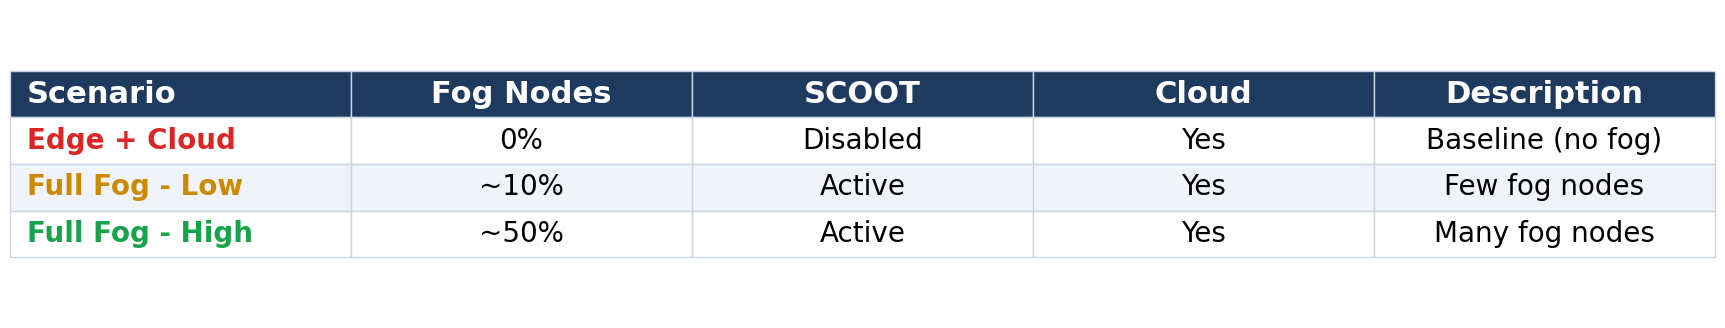
\includegraphics[width=0.95\textwidth,height=0.35\textheight,keepaspectratio]{table1_scenarios.png}
\end{center}

\vspace{0.2cm}
\textbf{Principe de comparaison \'equitable :}
\begin{itemize}
    \item M\^eme d\'ebit de trafic (2000 v\'eh/h) et m\^emes routes pour tous les sc\'enarios
    \item Seule la \textbf{densit\'e de fog nodes} varie entre les sc\'enarios
    \item Les diff\'erences de latence observ\'ees sont \textbf{uniquement dues au fog}
\end{itemize}
\end{frame}

\begin{frame}{Strat\'egie d'Offloading Multi-Crit\`eres}
\textbf{Mod\`ele math\'ematique de d\'ecision :}

\begin{equation}
\text{destination}^{*} = \arg\min_{d \in \{\text{local, fog, rsu, cloud}\}} \left( T_d + \alpha \cdot L_d + \beta \cdot E_d \right)
\end{equation}

O\`u : $T_d$ = temps d'ex\'ecution, $L_d$ = latence r\'eseau, $E_d$ = co\^ut \'energ\'etique

\vspace{0.2cm}
\textbf{Temps total d'offloading :}
\begin{align}
T_{\text{offload}} &= T_{\text{upload}} + T_{\text{exec}} + T_{\text{download}} \\
T_{\text{upload}} &= \frac{D_{\text{input}}}{BW_{\text{up}}}, \quad T_{\text{exec}} = \frac{I}{MIPS_d}, \quad T_{\text{download}} = \frac{D_{\text{output}}}{BW_{\text{down}}}
\end{align}

\textbf{Coefficients de pond\'eration :}
\begin{itemize}
    \item $W_{\text{latency}} = 0.35$ \quad $W_{\text{task\_size}} = 0.25$ \quad $W_{\text{congestion}} = 0.25$ \quad $W_{\text{fog\_avail}} = 0.15$
\end{itemize}
\end{frame}

\begin{frame}{M\'ecanisme de Capacit\'e RSU et Overflow}
\textbf{R\`egle cl\'e : Chaque RSU a une capacit\'e limit\'ee ($\sim$8 v\'ehicules simultan\'es)}

\vspace{0.2cm}
\textbf{Latence dynamique V2V (fog) en fonction de la densit\'e :}
\begin{equation}
L_{\text{V2V}} = \max\left(5, \; 20 - \rho_{\text{fog}} \times 30\right) \quad \text{ms}
\end{equation}

\textbf{Latence dynamique RSU :}
\begin{equation}
L_{\text{RSU}} = \max\left(7, \; 15 - \rho_{\text{fog}} \times 8\right) + \frac{d_{\text{RSU}}}{300} \times 5 \quad \text{ms}
\end{equation}

O\`u $\rho_{\text{fog}} = \frac{\text{fog\_nodes}}{\text{total\_v\'ehicules}}$ est la densit\'e fog et $d_{\text{RSU}}$ la distance au RSU.

\vspace{0.2cm}
\begin{alertblock}{M\'ecanisme d'overflow}
\begin{enumerate}
    \item RSU pas surcharg\'e $\rightarrow$ \textbf{RSU} (7-15 ms)
    \item RSU surcharg\'e + fog nearby $\rightarrow$ \textbf{FOG\_VEHICLE} (5-20 ms)
    \item RSU surcharg\'e + pas de fog $\rightarrow$ \textbf{CLOUD} (250 ms) $\leftarrow$ \textit{p\'enalit\'e massive}
\end{enumerate}
\end{alertblock}
\end{frame}

\begin{frame}[fragile]{Code : D\'ecision d'Offloading (iFogSim/Java)}
\begin{lstlisting}[style=java, title={VehicularFogSimulation.java -- calculateOffloadingDecision()}]
// RSU surcharge si >8 vehicules dans la zone
boolean rsuOverloaded = congestionNorm > 0.32;
double fogDensityRatio = (totalVehicles > 0) ? 
    (double) fogNodes / totalVehicles : 0.0;

// Latences dynamiques
double dynamicV2VLatency = Math.max(5.0, 20.0 - fogDensityRatio * 30.0);
double dynamicRSULatency = Math.max(7.0, 15.0 - fogDensityRatio * 8.0);
if (rsuOverloaded) {
    dynamicRSULatency *= (1.0 + congestionNorm * 2.0); // Penalite surcharge
}
double L_cloud = LATENCY_CLOUD * 2 + 150.0; // ~250ms

// Decision basee sur capacite RSU
if (cpuLoad < CPU_THRESHOLD_LOW && taskSizeNorm < 0.3)
    bestDest = "LOCAL";                    // Petite tache -> local (3ms)
else if (isInRSUZone && !rsuOverloaded)
    bestDest = "RSU";                      // RSU dispo -> RSU (7-15ms)
else if (hasFogVehicleNearby)
    bestDest = "FOG_VEHICLE";              // Fog nearby -> V2V (5-20ms)
else
    bestDest = "CLOUD";                    // Dernier recours -> Cloud (250ms)
\end{lstlisting}
\end{frame}

\begin{frame}{Outils et Algorithmes Utilis\'es}
\begin{table}
\centering
\begin{tabular}{lp{8cm}}
\toprule
\textbf{Outil} & \textbf{R\^ole dans la simulation} \\
\midrule
\textbf{SUMO} & Simulateur microscopique de trafic routier. G\`ere les v\'ehicules, feux et routes via l'API TraCI. \\
\textbf{iFogSim} & Simulateur Fog Computing (Java). Calcule les d\'ecisions d'offloading et les m\'etriques. \\
\textbf{Python/Flask} & Orchestrateur central + Dashboard temps r\'eel (Socket.IO). \\
\textbf{SCOOT} & Algorithme adaptatif de contr\^ole des feux (Split, Cycle, Offset). \\
\textbf{TraCI} & API Python pour contr\^oler SUMO en temps r\'eel. \\
\bottomrule
\end{tabular}
\end{table}

\vspace{0.2cm}
\textbf{Communication inter-composants :}
\begin{center}
\footnotesize
SUMO $\xleftrightarrow{\text{TraCI (Python)}}$ Orchestrateur (server.py) $\xleftrightarrow{\text{Socket TCP 5555}}$ iFogSim (Java)
\end{center}
\end{frame}

\begin{frame}[fragile]{Algorithme SCOOT Adaptatif}
\textbf{SCOOT} (Split Cycle Offset Optimization Technique) -- Contr\^ole adaptatif des feux :

\begin{columns}
\column{0.5\textwidth}
\textbf{Principe :}
\begin{itemize}
    \item Mesure des files d'attente en temps r\'eel
    \item Ajustement dynamique des phases de feux
    \item Optimisation par zone RSU
    \item 3 types de d\'ecisions : \textbf{split}, \textbf{cycle}, \textbf{offset}
\end{itemize}

\column{0.5\textwidth}
\begin{lstlisting}[style=java, title={SCOOTController.java}]
// Calcul du split optimal
double nsRatio = nsQueue / 
    (nsQueue + ewQueue + 1);
int nsGreen = (int)(cycleLength 
    * nsRatio);
int ewGreen = cycleLength - nsGreen;

// Seuils d'intervention
if (nsQueue > ewQueue * 1.5) {
  decision = "BASCULER vers N-S";
}
\end{lstlisting}
\end{columns}

\vspace{0.2cm}
\textbf{Formule du Performance Index (PI) :}
\begin{equation}
PI = \frac{Q_{\text{max}}}{Q_{\text{capacity}}} \quad \text{o\`u } Q_{\text{max}} = \max(Q_{NS}, Q_{EW})
\end{equation}
\end{frame}

\begin{frame}[fragile]{Code : Configuration SUMO et TraCI}
\begin{columns}
\column{0.5\textwidth}
\begin{lstlisting}[style=xml, title={routes\_low\_fog.rou.xml (10\% fog)}]
<!-- Types de vehicules -->
<vType id="car" maxSpeed="50" 
       guiShape="passenger" 
       color="0,0,255"/>
<vType id="fog_capable" maxSpeed="55" 
       guiShape="passenger/sedan" 
       color="0,255,0"/>

<!-- Route WE: 500 veh/h -->
<!-- 90% car, 10% fog -->
<flow id="we_car" type="car" 
      route="route_we" 
      begin="0" end="300" 
      vehsPerHour="450"/>
<flow id="we_fog" type="fog_capable" 
      route="route_we" 
      begin="0" end="300" 
      vehsPerHour="50"/>
\end{lstlisting}

\column{0.5\textwidth}
\begin{lstlisting}[style=python, title={server.py -- TraCI (Python)}]
import traci

# Connexion SUMO via TraCI
traci.start(["sumo-gui", "-c", 
    sumo_config_path])

# Boucle de simulation
while traci.simulation.getTime() < 300:
    traci.simulationStep()
    
    # Recuperer les vehicules
    for veh_id in traci.vehicle\
            .getIDList():
        x, y = traci.vehicle\
            .getPosition(veh_id)
        speed = traci.vehicle\
            .getSpeed(veh_id)
        vtype = traci.vehicle\
            .getTypeID(veh_id)
        
    # Changer les feux (SCOOT)
    traci.trafficlight.setPhase(
        tl_id, new_phase)
\end{lstlisting}
\end{columns}
\end{frame}

% ############################################
% SECTION 4 : PARAMETRES DE SIMULATION
% ############################################
\section{Param\`etres de Simulation}

\begin{frame}{Param\`etres de Simulation}
\begin{columns}
\column{0.5\textwidth}
\begin{center}
{\scriptsize\textbf{Network Infrastructure}}\\
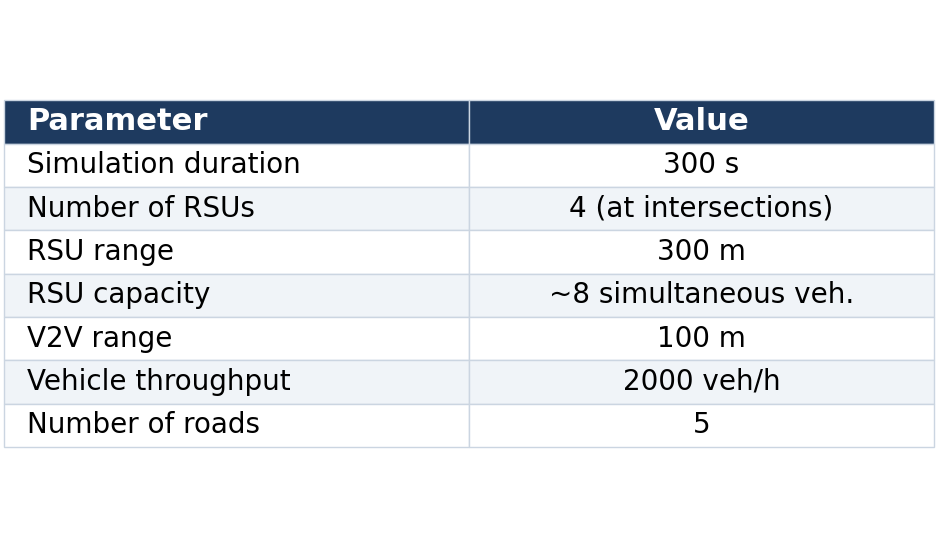
\includegraphics[width=\textwidth,height=0.38\textheight,keepaspectratio]{table2a_infrastructure.png}
\end{center}
\vspace{-0.2cm}
\begin{center}
{\scriptsize\textbf{Computing Capacities}}\\
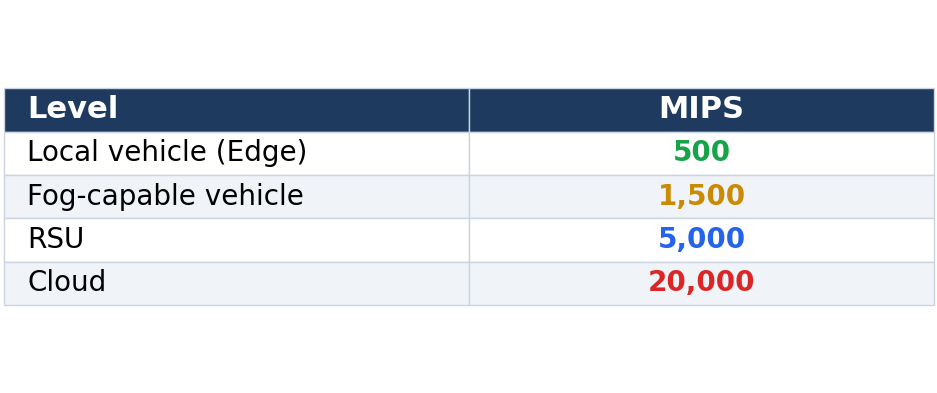
\includegraphics[width=\textwidth,height=0.34\textheight,keepaspectratio]{table2c_capacites.png}
\end{center}
\column{0.5\textwidth}
\begin{center}
{\scriptsize\textbf{Generated Tasks}}\\
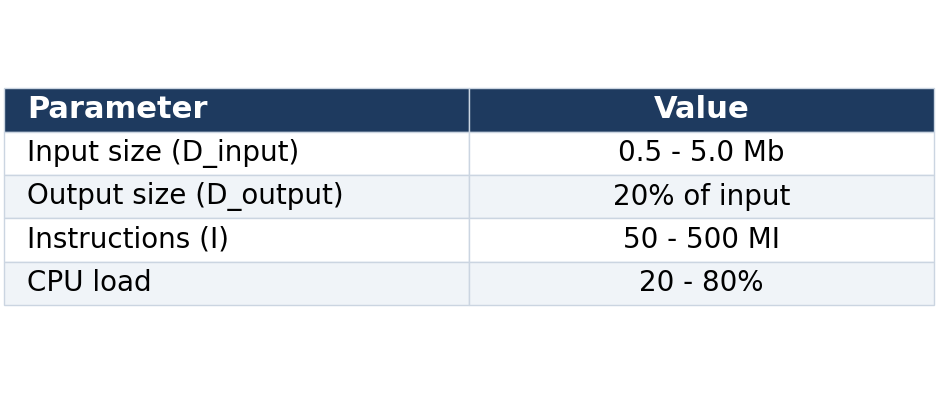
\includegraphics[width=\textwidth,height=0.34\textheight,keepaspectratio]{table2b_taches.png}
\end{center}
\vspace{-0.2cm}
\begin{center}
{\scriptsize\textbf{Bandwidth and Latency}}\\
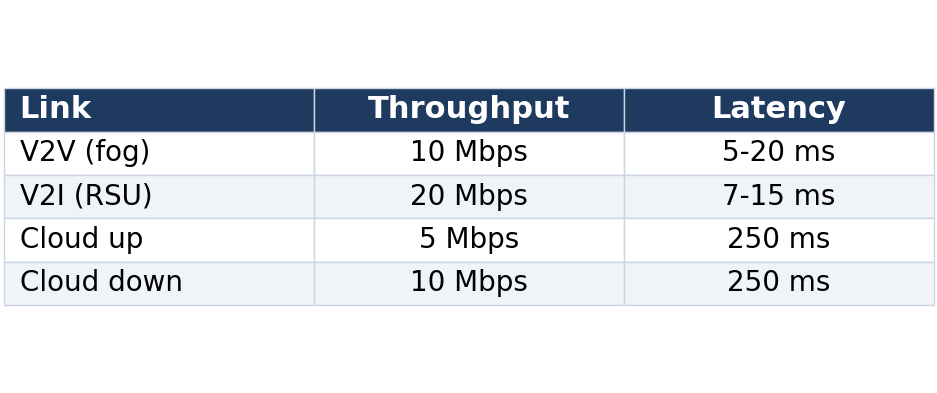
\includegraphics[width=\textwidth,height=0.34\textheight,keepaspectratio]{table2d_bandes.png}
\end{center}
\end{columns}
\end{frame}

\begin{frame}{D\'etail des Sc\'enarios de Trafic}
\begin{center}
{\small\textbf{Traffic Scenario Details}}\\[0.1cm]
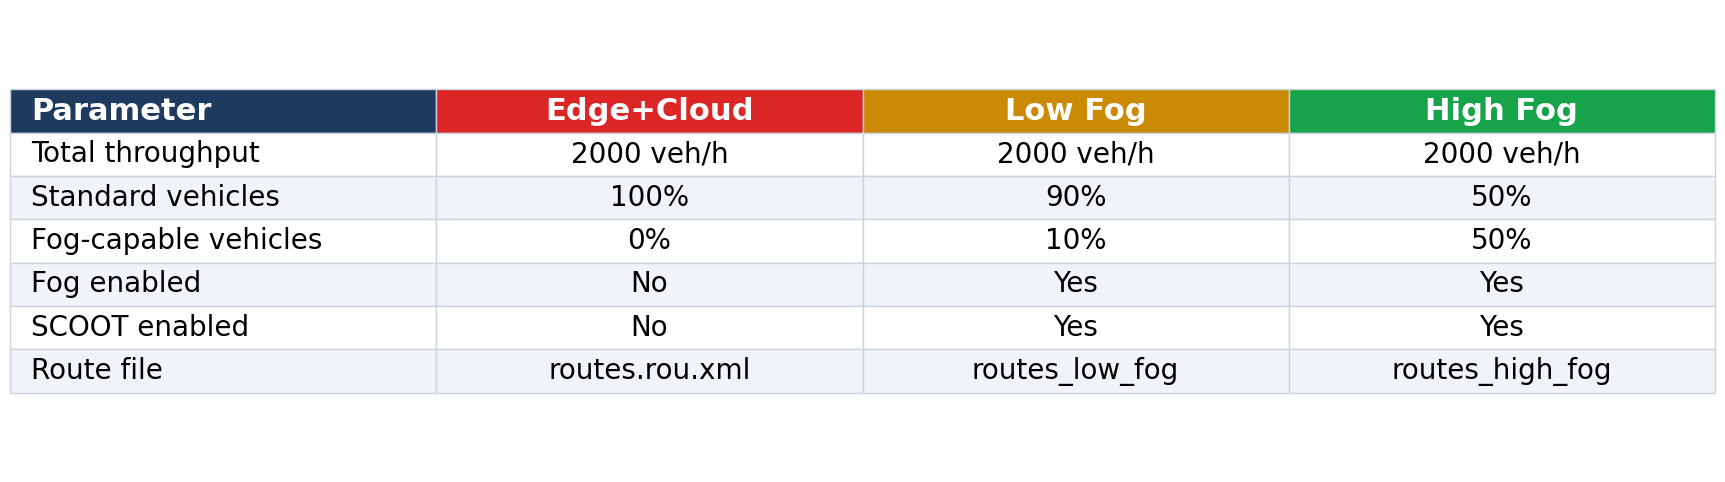
\includegraphics[width=0.95\textwidth,height=0.45\textheight,keepaspectratio]{table3_scenarios_detail.png}
\end{center}

\vspace{0.3cm}
\textbf{Co\^uts \'energ\'etiques :}
\begin{itemize}
    \item Calcul local : $E_{\text{compute}} = I \times 0.5$ J/MI
    \item Calcul fog : $E_{\text{compute}} = I \times 0.1$ J/MI
    \item Transmission : $E_{\text{transmit}} = (D_{\text{in}} + D_{\text{out}}) \times 0.01$ J/Mb
\end{itemize}
\end{frame}

% ############################################
% SECTION 5 : METRIQUES EVALUEES
% ############################################
\section{M\'etriques \'Evalu\'ees}

\begin{frame}{M\'etriques \'Evalu\'ees}
\begin{center}
{\small\textbf{Evaluated Metrics}}\\[0.1cm]
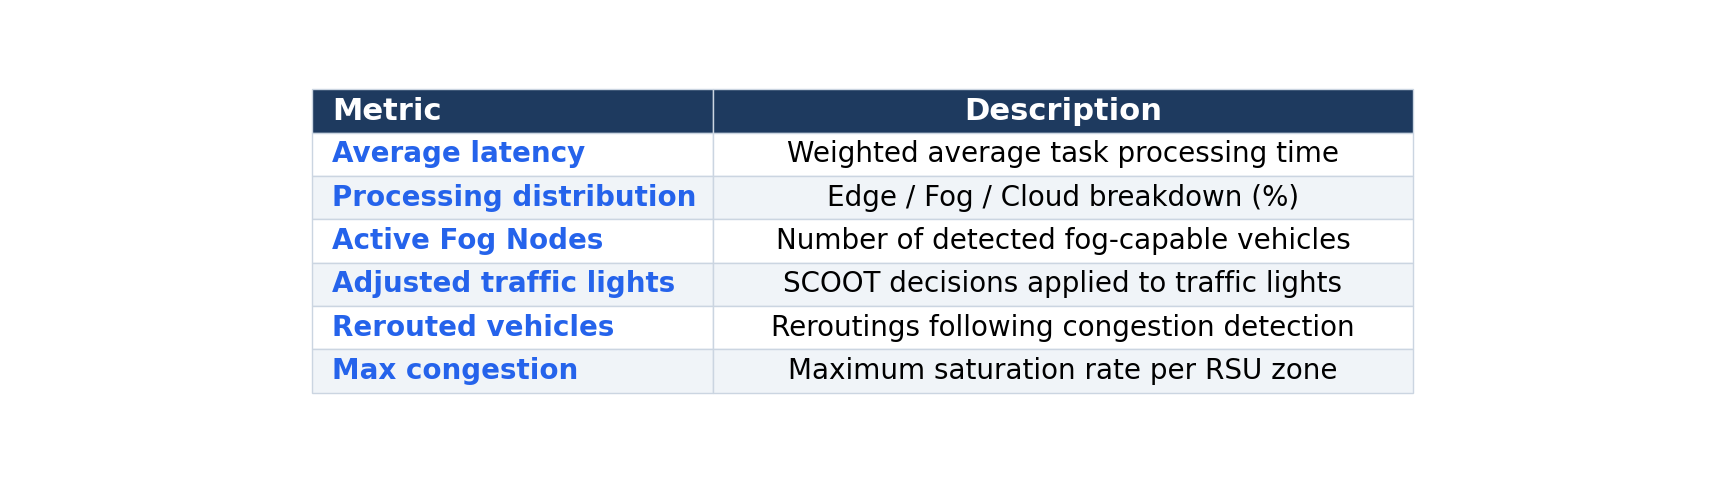
\includegraphics[width=0.95\textwidth,height=0.5\textheight,keepaspectratio]{table4_metriques.png}
\end{center}
\end{frame}

\begin{frame}{Formules des M\'etriques}
\textbf{Formule de la latence moyenne pond\'er\'ee :}
\begin{equation}
L_{\text{avg}} = \frac{L_{\text{edge}} \times P_{\text{edge}} + L_{\text{fog}} \times P_{\text{fog}} + L_{\text{cloud}} \times P_{\text{cloud}}}{100}
\end{equation}

O\`u $P_{\text{edge}} + P_{\text{fog}} + P_{\text{cloud}} = 100\%$ repr\'esente la distribution du traitement.

\vspace{0.3cm}
\textbf{Niveau de congestion par zone :}
\begin{equation}
C_{\text{zone}} = \min\left(1, \; \frac{N_{\text{v\'ehicules\_zone}}}{25}\right) \quad \text{(25+ v\'ehicules = 100\% congestion)}
\end{equation}
\end{frame}

% ############################################
% SECTION 6 : RESULTATS OBTENUS
% ############################################
\section{R\'esultats Obtenus}

\begin{frame}{R\'esultats : Tableau Comparatif}
\begin{center}
{\small\textbf{Comparative Results}}\\[0.1cm]
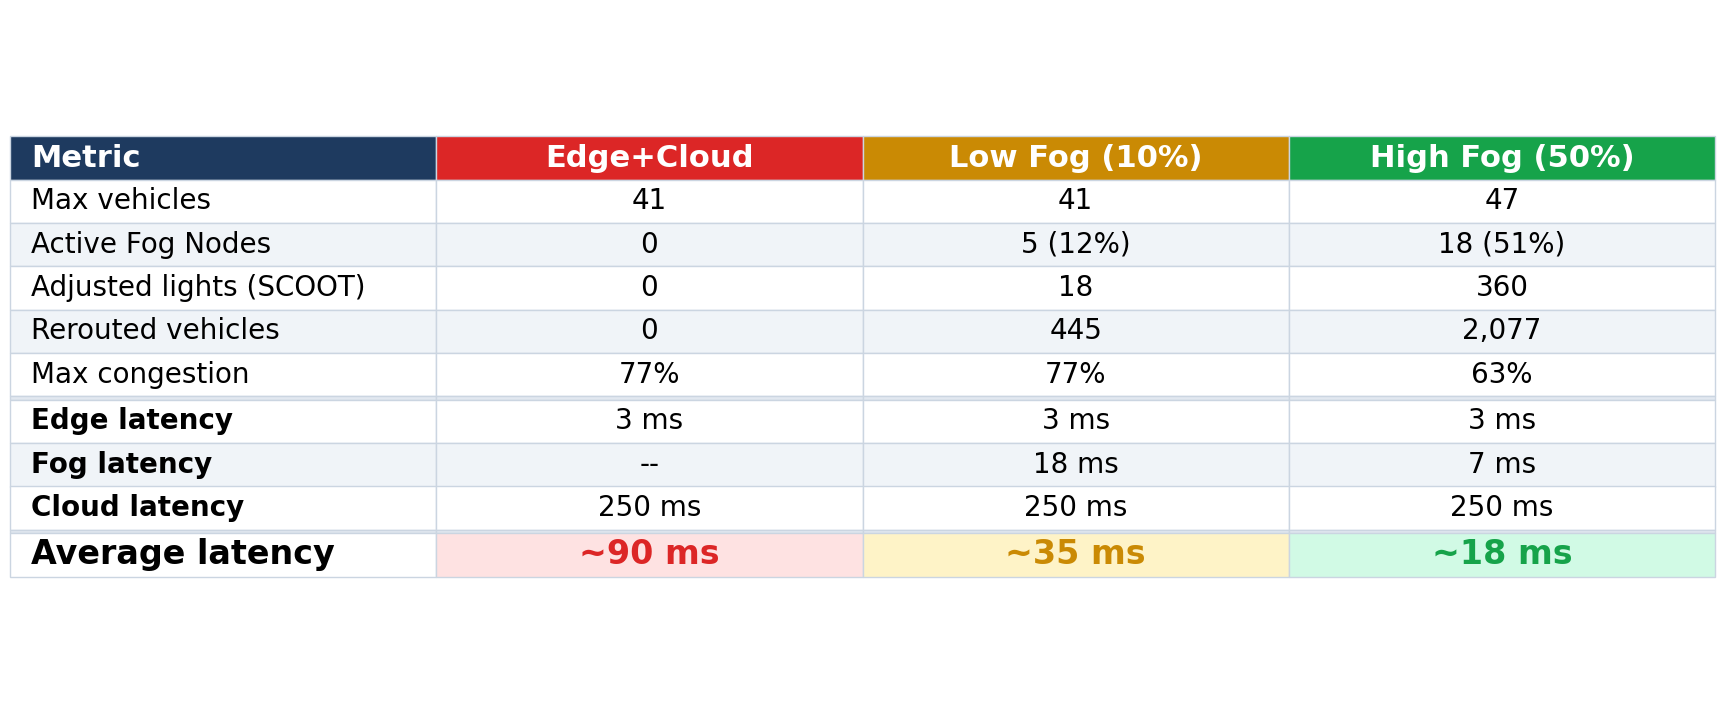
\includegraphics[width=0.95\textwidth,height=0.65\textheight,keepaspectratio]{table5_resultats.png}
\end{center}

\begin{block}{Observation cl\'e}
Le Fog Computing r\'eduit la latence de \textbf{61\%} (Low Fog) \`a \textbf{80\%} (High Fog) par rapport au Cloud seul.
\end{block}
\end{frame}

\begin{frame}{R\'esultats : Latence Moyenne par Sc\'enario}
\begin{center}
{\small\textbf{Average Latency per Scenario}}\\[0.1cm]
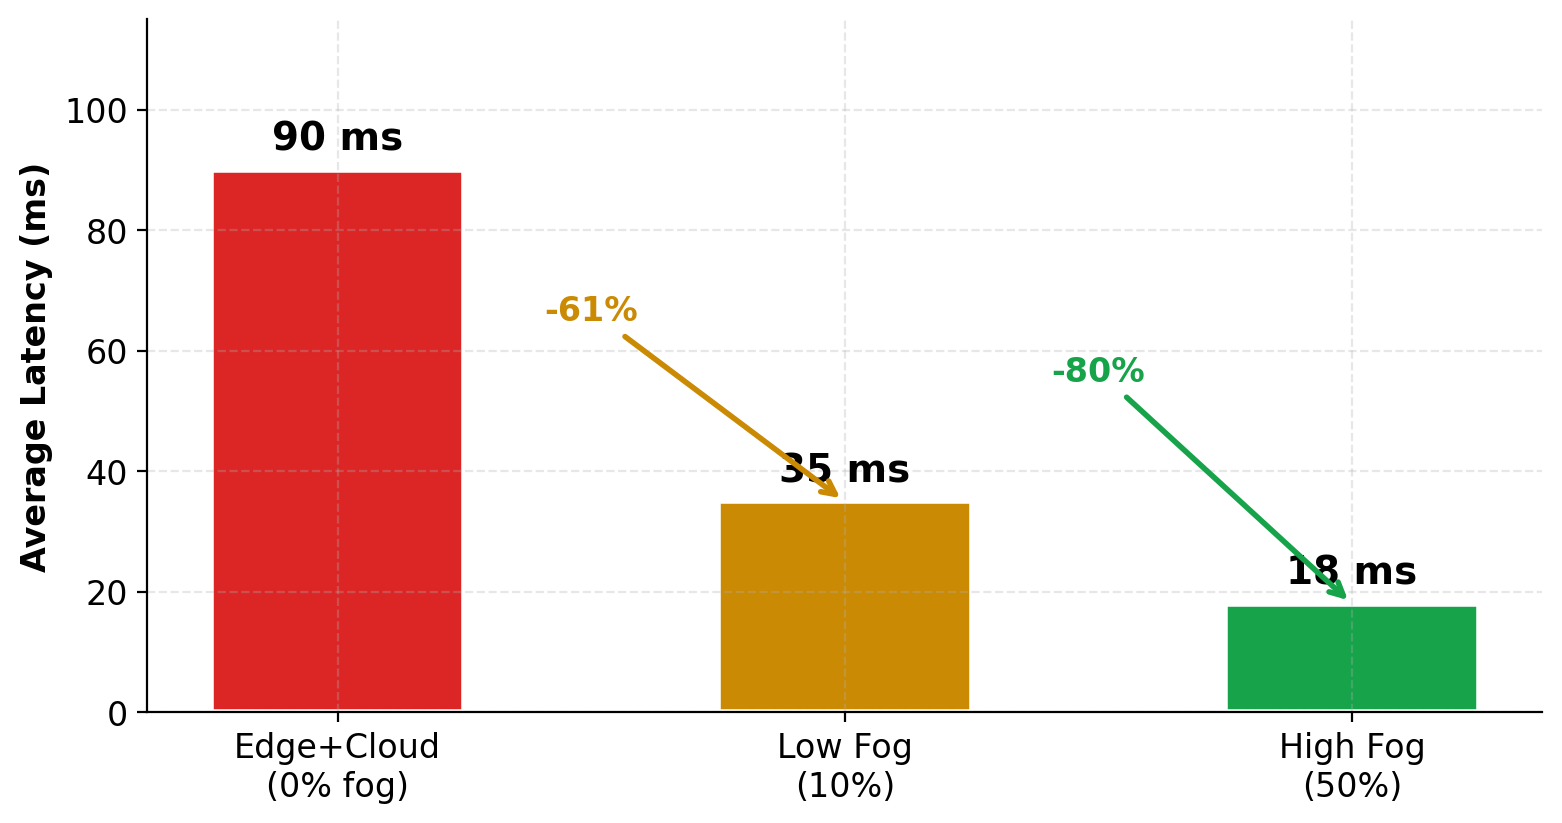
\includegraphics[width=0.9\textwidth,height=0.6\textheight,keepaspectratio]{plot1_latence_moyenne.png}
\end{center}

\textbf{R\'eduction :} Low Fog : \textcolor{foggreen}{-61\%} (90$\rightarrow$35 ms) \quad High Fog : \textcolor{foggreen}{-80\%} (90$\rightarrow$18 ms)
\end{frame}

\begin{frame}{R\'esultats : \'Evolution de la Latence}
\begin{center}
{\small\textbf{Latency Evolution vs. Number of Vehicles}}\\[0.1cm]
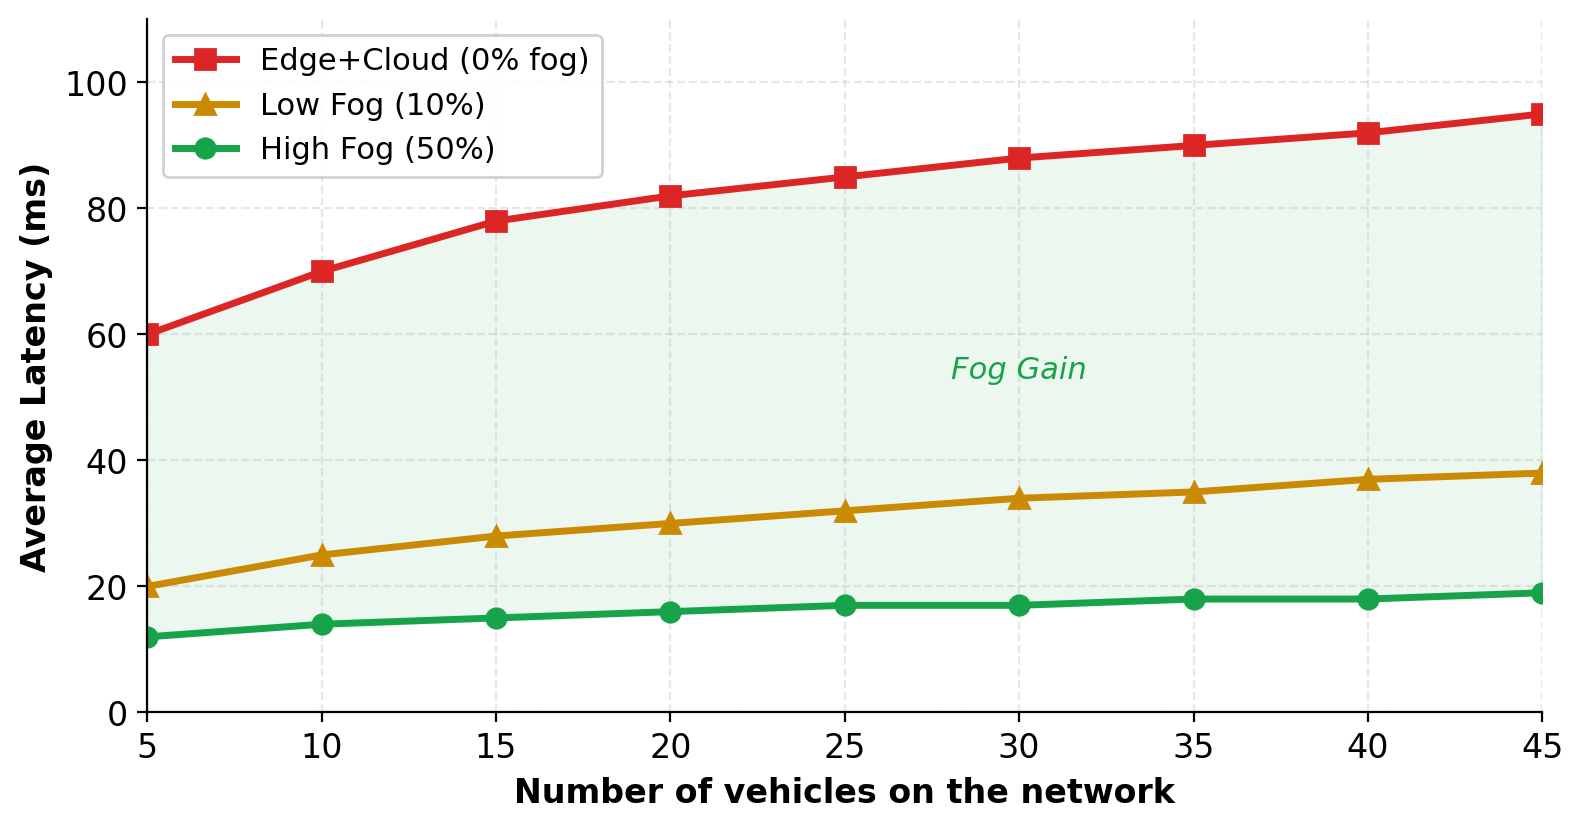
\includegraphics[width=0.9\textwidth,height=0.63\textheight,keepaspectratio]{plot2_evolution_latence.png}
\end{center}

\textbf{Observation :} Plus le nombre de v\'ehicules augmente, plus l'\'ecart de latence se creuse entre les sc\'enarios. Le fog maintient une latence stable.
\end{frame}

\begin{frame}{R\'esultats : Distribution du Traitement}
\begin{center}
{\small\textbf{Processing Distribution per Scenario}}\\[0.1cm]
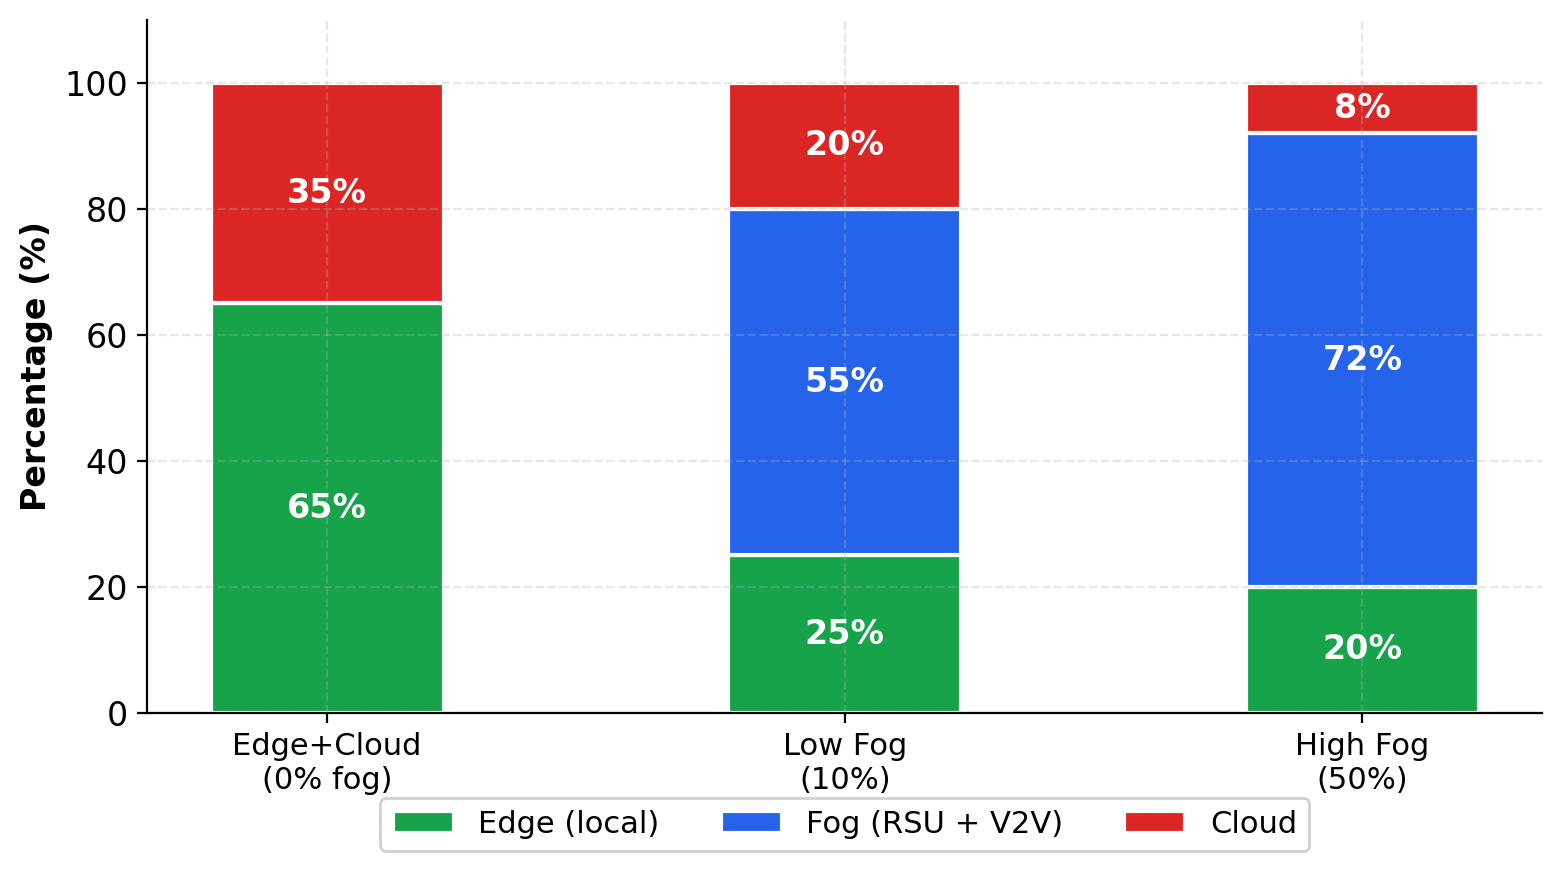
\includegraphics[width=0.9\textwidth,height=0.63\textheight,keepaspectratio]{plot3_distribution.png}
\end{center}

\textbf{Interpr\'etation :} Avec 50\% de fog nodes, \textbf{72\%} des t\^aches sont trait\'ees localement par le fog, r\'eduisant l'usage du cloud de 35\% \`a 8\%.
\end{frame}

\begin{frame}{R\'esultats : Actions Fog (Feux Ajust\'es et Reroutages)}
\begin{center}
{\small\textbf{Fog Actions: Adjusted Lights \& Rerouted Vehicles}}\\[0.1cm]
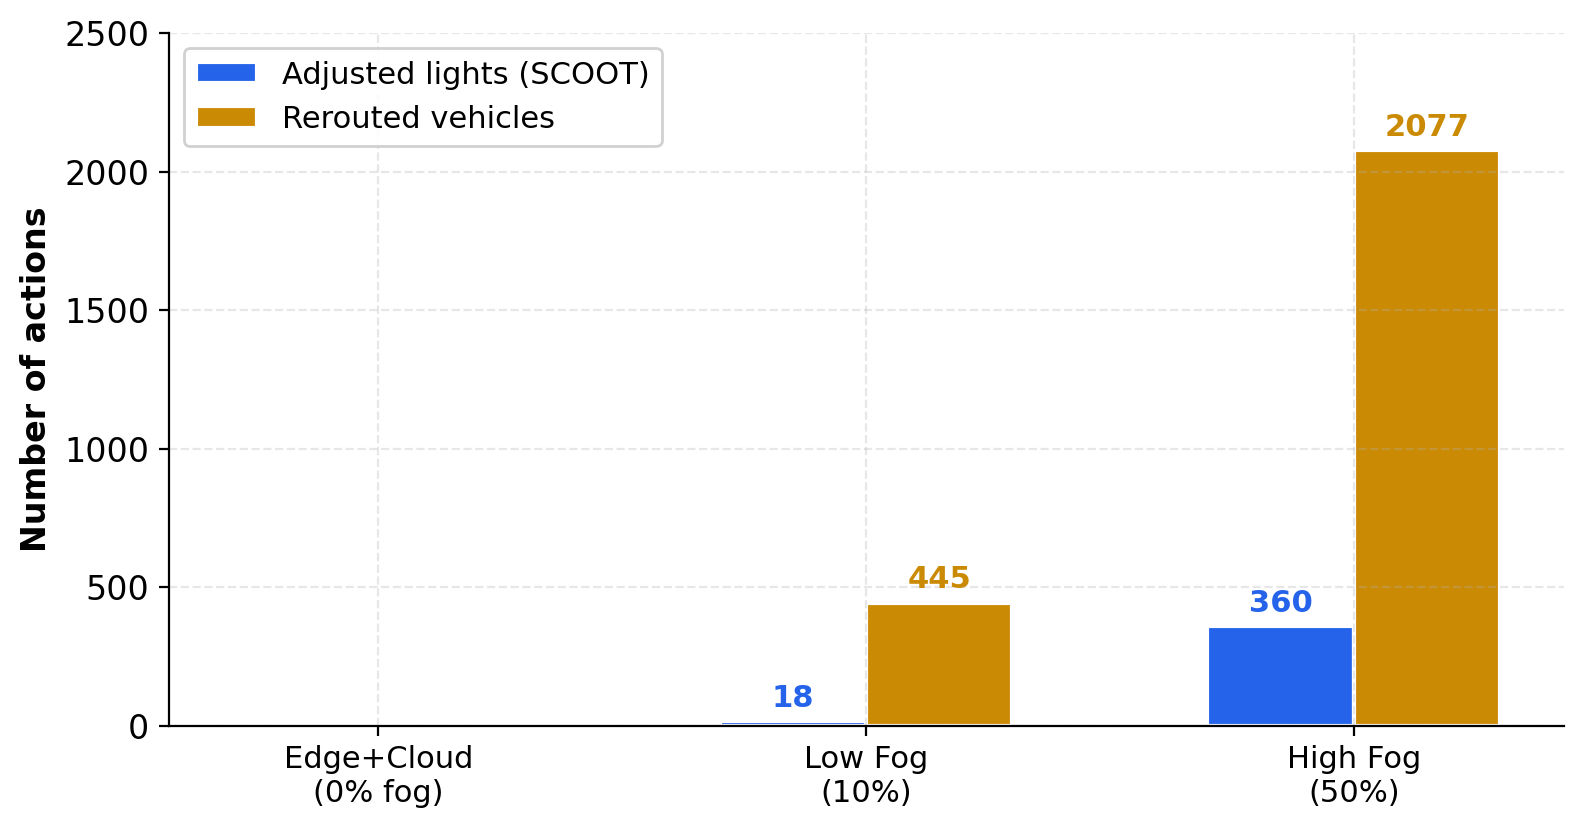
\includegraphics[width=0.9\textwidth,height=0.63\textheight,keepaspectratio]{plot4_actions_fog.png}
\end{center}

\textbf{Impact du Fog :} Plus de fog nodes $\Rightarrow$ plus de d\'ecisions locales, plus de r\'eactivit\'e. SCOOT ajuste \textbf{20$\times$ plus de feux} en High Fog.
\end{frame}

\begin{frame}[fragile]{R\'esultats : Exemples de D\'ecisions SCOOT en Temps R\'eel}
\textbf{D\'ecisions SCOOT observ\'ees (High Fog, T=60-120s) :}

\begin{lstlisting}[style=bash]
[SCOOT SPLIT] J2: EW=32s, NS=18s (PI=0.00, NS queue=0m, EW queue=7m)
[EXEC FOG->SUMO] J1: BASCULE vers N-S - NS:5 EW:0
[EXEC FOG->SUMO] RSU_J1: 25 vehicules REROUTES
[EXEC FOG->SUMO] J2: Vert E-W etendu a 40s
[EXEC FOG->SUMO] J3: Vert N-S etendu a 40s
\end{lstlisting}

\vspace{0.2cm}
\textbf{Interpr\'etation :}
\begin{itemize}
    \item \textbf{PI} (Performance Index) : 0 = fluide, 1 = bloqu\'e
    \item \textbf{Split} : R\'epartition du temps de vert (ex: NS=18s, EW=32s)
    \item \textbf{Reroutage} : 25 v\'ehicules redirig\'es pour \'eviter la congestion
    \item \textbf{Extension} : Phase verte \'etendue si file d'attente importante
    \item Toutes les d\'ecisions prises en \textbf{$<$ 50 ms} gr\^ace au traitement fog local
\end{itemize}
\end{frame}

% ############################################
% SECTION 7 : DEMONSTRATION
% ############################################
\section{D\'emonstration}

\begin{frame}{D\'emonstration en Direct}
\centering
\Large\textbf{Lancement des 3 sc\'enarios de simulation}

\vspace{0.5cm}
\begin{columns}
\column{0.33\textwidth}
\centering
\textcolor{red}{\rule{2cm}{3pt}}\\
\vspace{0.2cm}
{\large\textbf{Sc\'enario 1}}\\
\vspace{0.1cm}
\textbf{Edge + Cloud}\\
(0\% fog)\\
\vspace{0.2cm}
{\small\textit{R\'ef\'erence}}\\
{\small SCOOT d\'esactiv\'e}\\
{\small Cloud seul ($\sim$250 ms)}

\column{0.33\textwidth}
\centering
\textcolor{orange}{\rule{2cm}{3pt}}\\
\vspace{0.2cm}
{\large\textbf{Sc\'enario 2}}\\
\vspace{0.1cm}
\textbf{Low Fog}\\
(10\% fog nodes)\\
\vspace{0.2cm}
{\small\textit{Fog limit\'e}}\\
{\small SCOOT actif}\\
{\small Latence $\sim$35 ms}

\column{0.33\textwidth}
\centering
\textcolor{green!60!black}{\rule{2cm}{3pt}}\\
\vspace{0.2cm}
{\large\textbf{Sc\'enario 3}}\\
\vspace{0.1cm}
\textbf{High Fog}\\
(50\% fog nodes)\\
\vspace{0.2cm}
{\small\textit{Fog dense}}\\
{\small SCOOT actif}\\
{\small Latence $\sim$18 ms}
\end{columns}

\vspace{0.5cm}
\begin{alertblock}{\`A observer}
Dashboard temps r\'eel $\bullet$ Ajustements SCOOT $\bullet$ Reroutages $\bullet$ Latence $\bullet$ Distribution du traitement
\end{alertblock}
\end{frame}

% ############################################
% SECTION 8 : DISCUSSION
% ############################################
\section{Discussion}

\begin{frame}{Discussion des R\'esultats}
\textbf{Observations principales :}

\begin{enumerate}
    \item \textbf{R\'eduction de latence significative} : jusqu'\`a 80\% avec High Fog
    \begin{itemize}
        \item Le fog absorbe l'overflow RSU (5-20 ms vs 250 ms cloud)
        \item Plus de fog nodes = meilleure couverture V2V = moins de cloud
    \end{itemize}
    
    \item \textbf{SCOOT beaucoup plus efficace avec le fog}
    \begin{itemize}
        \item High Fog : 360 ajustements vs Edge+Cloud : 0 ajustement
        \item La latence r\'eduite permet des d\'ecisions plus fr\'equentes
    \end{itemize}
    
    \item \textbf{Gestion proactive de la congestion}
    \begin{itemize}
        \item 2077 reroutages en High Fog vs 0 en Edge+Cloud
        \item Congestion max r\'eduite de 77\% \`a 63\% gr\^ace au fog
    \end{itemize}
    
    \item \textbf{R\'esultat contre-intuitif} : High Fog a une congestion \textbf{plus basse}
    \begin{itemize}
        \item Le SCOOT + reroutage anticipe et distribue le trafic
    \end{itemize}
\end{enumerate}
\end{frame}

\begin{frame}{Avantages et Limites du Fog V\'ehiculaire}
\begin{columns}
\column{0.5\textwidth}
\textbf{Avantages d\'emontr\'es :}
\begin{itemize}
    \item[$\checkmark$] Latence r\'eduite : 90 ms $\rightarrow$ 18 ms
    \item[$\checkmark$] D\'ecisions temps r\'eel ($<$ 50 ms)
    \item[$\checkmark$] Pas de point unique de d\'efaillance
    \item[$\checkmark$] \'Economie de bande passante cloud
    \item[$\checkmark$] Conscience du contexte local
    \item[$\checkmark$] Scalabilit\'e proportionnelle au trafic
\end{itemize}

\column{0.5\textwidth}
\textbf{Limites identifi\'ees :}
\begin{itemize}
    \item[$\times$] Performance d\'epend de la densit\'e fog
    \item[$\times$] Mobilit\'e = voisins fog instables
    \item[$\times$] H\'et\'erog\'en\'eit\'e des ressources v\'ehiculaires
    \item[$\times$] N\'ecessite infrastructure RSU
    \item[$\times$] S\'ecurit\'e et authentification complexes
    \item[$\times$] Pas de fog en zones rurales peu denses
\end{itemize}
\end{columns}

\vspace{0.3cm}
\begin{alertblock}{Seuil d'efficacit\'e}
\`A partir de $\sim$10\% de fog nodes, les b\'en\'efices sont significatifs (-61\% latence). Le passage \`a 50\% apporte un gain suppl\'ementaire (-80\%).
\end{alertblock}
\end{frame}

% ############################################
% SECTION 8 : CONCLUSION ET PERSPECTIVES
% ############################################
\section{Conclusion et Perspectives}

\begin{frame}{Conclusion}
\textbf{Ce que nous avons d\'emontr\'e :}

\begin{enumerate}
    \item Le \textbf{Fog Computing} r\'eduit la latence de \textbf{80\%} (90 $\rightarrow$ 18 ms)
    \item L'algorithme \textbf{SCOOT} optimise les feux en temps r\'eel (360 ajustements)
    \item Le m\'ecanisme de \textbf{capacit\'e RSU} avec overflow vers fog/cloud cr\'ee une diff\'erenciation r\'ealiste
    \item Plus de \textbf{fog nodes} = meilleure gestion du trafic et congestion r\'eduite
    \item L'architecture \textbf{Edge-Fog-Cloud} est efficace et scalable pour les VANET
\end{enumerate}

\vspace{0.3cm}
\begin{block}{Message cl\'e}
Le Fog Computing V\'ehiculaire n'est pas une alternative au Cloud, mais un \textbf{compl\'ement essentiel} qui rapproche le calcul des v\'ehicules. Il permet des d\'ecisions en \textbf{temps r\'eel} l\`a o\`u le Cloud \'echoue.
\end{block}
\end{frame}

\begin{frame}{Perspectives}
\textbf{Am\'eliorations futures :}

\begin{itemize}
    \item \textbf{Machine Learning} : Pr\'ediction de congestion par mod\`eles ML (LSTM, GNN)
    \item \textbf{5G/6G C-V2X} : Int\'egration pour latence $<$ 1 ms
    \item \textbf{Federated Learning} : Apprentissage distribu\'e coop\'eratif sur v\'ehicules
    \item \textbf{S\'ecurit\'e} : PKI v\'ehiculaire (IEEE 1609.2)
    \item \textbf{Platooning} : Application aux convois de camions autonomes
    \item \textbf{Multi-hop V2V} : Extension de la port\'ee fog par relais
\end{itemize}

\vspace{0.3cm}
\textbf{\'Evolution technologique :}
\begin{center}
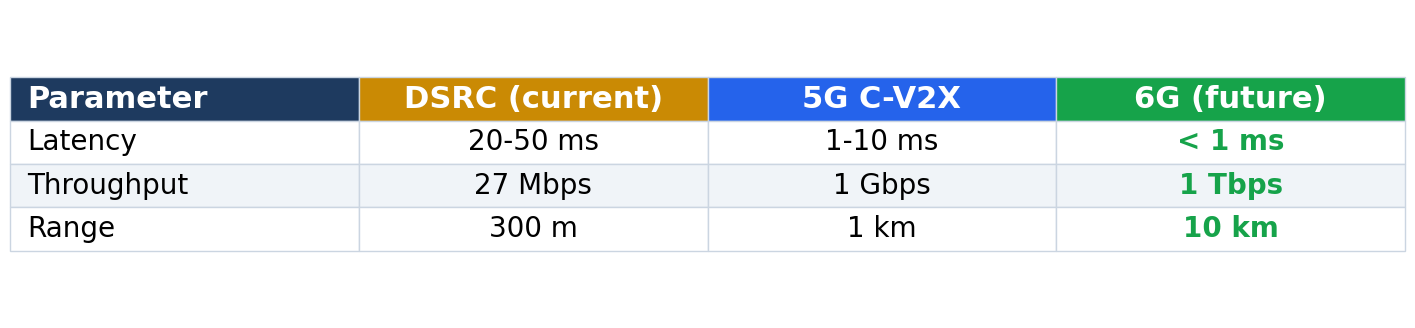
\includegraphics[width=0.9\textwidth,height=0.3\textheight,keepaspectratio]{table6_evolution.png}
\end{center}
\end{frame}

\begin{frame}{R\'ef\'erences}
\footnotesize
\begin{thebibliography}{9}
\bibitem{bonomi2012} Bonomi, F. et al. (2012). ``Fog Computing and Its Role in the Internet of Things.'' MCC Workshop, ACM.

\bibitem{hou2016} Hou, X. et al. (2016). ``Vehicular Fog Computing: A Viewpoint of Vehicles as the Infrastructures.'' IEEE VTC.

\bibitem{ifogsim} Gupta, H. et al. (2017). iFogSim: A toolkit for modeling and simulation of resource management techniques in IoT, Edge and Fog computing.

\bibitem{scoot} Hunt, P.B. et al. (1981). ``SCOOT -- A Traffic Responsive Method of Coordinating Signals.'' TRRL Report.

\bibitem{sumo} Lopez, P.A. et al. (2018). ``Microscopic Traffic Simulation using SUMO.'' IEEE ITSC.
\end{thebibliography}
\end{frame}

\begin{frame}
\centering
\Huge\textbf{Merci pour votre attention}

\vspace{1cm}
\Large Questions ?
\end{frame}

\end{document}

